\documentclass[conference]{article}
\usepackage{times}
\usepackage{icml2017} 
% numbers option provides compact numerical references in the text. 

\usepackage{multicol}
\usepackage[bookmarks=true]{hyperref}
\usepackage{amsmath,amssymb}

\usepackage{caption}
\usepackage{graphicx}
\usepackage{epstopdf}
\renewcommand{\captionfont}{\footnotesize}
\usepackage{sidecap,wrapfig}
\usepackage{subfigure}
%\usepackage[ruled,vlined]{algorithm2e}
\usepackage{times}
\usepackage{microtype}
\usepackage{tabularx}
\usepackage{tikz,hyperref,graphicx,units}
\usepackage{subfigure}
\usepackage{bbm}
%\renewcommand{\baselinestretch}{.5}


\renewcommand{\captionfont}{\footnotesize}
\usepackage{sidecap,wrapfig}
%\usepackage[ruled,vlined]{algorithm2e}

\DeclareMathOperator*{\argmin}{arg\,min}
\DeclareMathOperator*{\argmax}{arg\,max}
\newcommand{\abs}[1]{\lvert#1\rvert} 
\newcommand{\norm}[1]{\lVert#1\rVert}
%\newcommand{\suchthat}{\mid}
\newcommand{\suchthat}{\ \big|\ }
\newcommand{\ba}{\mathbf{a}}
\newcommand{\bs}{\mathbf{s}}
\newcommand{\bb}{\mathbf{b}}
\newcommand{\bc}{\mathbf{c}}
\newcommand{\bd}{\mathbf{d}}
\newcommand{\bg}{\mathbf{g}}
\newcommand{\bj}{\mathbf{j}}
\newcommand{\bn}{\mathbf{n}}
\newcommand{\bp}{\mathbf{p}}
\newcommand{\bw}{\mathbf{w}}
\newcommand{\bt}{\mathbf{t}}
\newcommand{\bu}{\mathbf{u}}
\newcommand{\by}{\mathbf{y}}
\newcommand{\bx}{\mathbf{x}}
\newcommand{\bz}{\mathbf{z}}
\newcommand{\bbf}{\mathbf{f}}
\newcommand{\bzero}{\mathbf{0}}
\newcommand{\bG}{\mathbf{G}}
\newcommand{\bA}{\mathbf{A}}
\newcommand{\bW}{\mathbf{W}}
\newcommand{\bX}{\mathbf{X}}
\newcommand{\mX}{\mathcal{X}}
\newcommand{\mD}{\mathcal{D}}
\newcommand{\mG}{\mathcal{G}}
\newcommand{\mN}{\mathcal{N}}
\newcommand{\mW}{\mathcal{W}}
\newcommand{\mF}{\mathcal{F}}
\newcommand{\bZ}{\mathbf{Z}}
\newcommand{\bbZ}{\mathbb{Z}}
\newcommand{\mR}{\mathcal{R}}

\newtheorem{theorem}{Theorem}[section]
\newtheorem{lemma}[theorem]{Lemma}
\newtheorem{proof}[theorem]{proof}
\newtheorem{proposition}[theorem]{Proposition}
\newtheorem{corollary}[theorem]{Corollary}
%\usepackage[ruled,vlined]{algorithm2e}
\usepackage{url}
\newenvironment{definition}[1][Definition]{\begin{trivlist}
\item[\hskip \labelsep {\bfseries #1}]}{\end{trivlist}}

%\newcommand{\qed}{\nobreak \ifvmode \relax \else
   %   \ifdim\lastskip<1.5em \hskip-\lastskip
     % \hskip1.5em plus0em minus0.5em \fi \nobreak
      %\vrule height0.75em width0.5em depth0.25em\fi}

\def\lc{\left\lfloor}   
\def\rc{\right\rfloor}

\usepackage{amsmath,amssymb}

\newcommand{\bfc}{W}
\newcommand{\Qinf}{Q_{\infty}}
\newcommand{\st}[1]{_\text{#1}}
\newcommand{\rres}{r\st{res}}
\newcommand{\pos}[1]{(#1)^+}
\newcommand{\depth}{\operatorname{depth}}
\newcommand{\dist}{\operatorname{dist}}
\newcommand{\convhull}{\operatorname{ConvexHull}}
\newcommand{\minksum}{\operatorname{MinkowskiSum}}

\newcommand{\specialcell}[2][c]{ \begin{tabular}[#1]{@{}c@{}}#2\end{tabular}}
\newcommand{\acro}{SHIV}
\newcommand{\ns}{HC }
\newcommand{\nc}{RC }
\newcommand\independent{\protect\mathpalette{\protect\independenT}{\perp}}
%\def\independenT#1#2{\mathrel{\rlap{$#1#2$}\mkern2mu{#1#2}}}

%\newtheorem{lemma}{Lemma}[section]
%\newtheorem{theorem}{Theorem}[section]
\newtheorem{defn}{Definition}[section]

\newboolean{include-notes}
\setboolean{include-notes}{true}
\newcommand{\adnote}[1]{\ifthenelse{ \boolean{include-notes}}%
 {\textcolor{blue}{\textbf{#1}}}{}}
 
 \newcommand{\sknote}[1]{\ifthenelse{ \boolean{include-notes}}%
 {\textcolor{blue}{\textbf{SK: #1}}}{}}
 
  \newcommand{\mlnote}[1]{\ifthenelse{ \boolean{include-notes}}%
 {\textcolor{purple}{\textbf{ML: #1}}}{}}
 
 \newcommand{\jmnote}[1]{\ifthenelse{ \boolean{include-notes}}%
 {\textcolor{orange}{\textbf{JM: #1}}}{}}

%\renewcommand{\baselinestretch}{.95}
%\usepackage{times}
%\usepackage{microtype}



\begin{document}

% paper title
\title{An Iterative Noise\\ Injection Algorithm  for Scalable\\ Distributed Off-Policy Imitation Learning}

% You will get a Paper-ID when submitting a pdf file to the conference system
\author{Author Names Omitted for Anonymous Review}

%\author{\authorblockN{Michael Shell}
%\authorblockA{School of Electrical and\\Computer Engineering\\
%Georgia Institute of Technology\\
%Atlanta, Georgia 30332--0250\\
%Email: mshell@ece.gatech.edu}
%\and
%\authorblockN{Homer Simpson}
%\authorblockA{Twentieth Century Fox\\
%Springfield, USA\\
%Email: homer@thesimpsons.com}
%\and
%\authorblockN{James Kirk\\ and Montgomery Scott}
%\authorblockA{Starfleet Academy\\
%San Francisco, California 96678-2391\\
%Telephone: (800) 555--1212\\
%Fax: (888) 555--1212}}


% avoiding spaces at the end of the author lines is not a problem with
% conference papers because we don't use \thanks or \IEEEmembership


% for over three affiliations, or if they all won't fit within the width
% of the page, use this alternative format:
% 
%\author{\authorblockN{Michael Shell\authorrefmark{1},
%Homer Simpson\authorrefmark{2},
%James Kirk\authorrefmark{3}, 
%Montgomery Scott\authorrefmark{3} and
%Eldon Tyrell\authorrefmark{4}}
%\authorblockA{\authorrefmark{1}School of Electrical and Computer Engineering\\
%Georgia Institute of Technology,
%Atlanta, Georgia 30332--0250\\ Email: mshell@ece.gatech.edu}
%\authorblockA{\authorrefmark{2}Twentieth Century Fox, Springfield, USA\\
%Email: homer@thesimpsons.com}
%\authorblockA{\authorrefmark{3}Starfleet Academy, San Francisco, California 96678-2391\\
%Telephone: (800) 555--1212, Fax: (888) 555--1212}
%\authorblockA{\authorrefmark{4}Tyrell Inc., 123 Replicant Street, Los Angeles, California 90210--4321}}


\maketitle

\begin{abstract}
In Imitation Learning a supervisor’s policy is observed and the intended behavior is learned via function approximation. It has been shown for long time horizon tasks there exists a problem of covariate shift, where the agent visits different states than the supervisor. While work has been done addressing this problem by rolling-out the current agent's policy, these on-policy approaches are potentially not amenable to large batch updates.  Large updates can cause the data collected from the current agent to be uninformative at the next iteration.  We theoretically demonstrate that this covariate shift can also be alleviated via the injection of artificial noise into each supervisor’s policy. We provide an algorithm that leverages our analysis to estimate the optimal level of noise to inject for an $\epsilon$-greedy noise distribution.  Results on a driving simulator, which learns an image to action neural network policy, indicate with a batch size of $150$ demonstrations collected in parallel, we can obtain a $X\%$ increase in cumulative reward over on-policy methods such as DAgger. 
\end{abstract}

%\IEEEpeerreviewmaketitle

\section{Introduction}

In Imitation Learning (IL), an agent learns to mimic a supervisor on a task involving sequential decisions~\cite{argall2009survey}.  The generality of this approach has lead to a wide range of applications: parsing sentence structure~\cite{ballesteros2016training}, playing video games~\cite{NIPS2014_5421}, robotic manipulation~\cite{laskey2016robot} and self-driving cars~\cite{pomerleau1989alvinn}. 



Similar to Reinforcement Learning, (IL) has two types of algorithms: Off-Policy and On-Policy. In Off-Policy IL, an agent observes demonstrations from a supervisor and tries to recover the behavior via supervised learning~\cite{pomerleau1989alvinn}. A problem with Off-Policy algorithms, is that the agent may not perfectly agree with the supervisor during training. These small errors can compound during execution of the agent's policy because the agent may deviate greatly from the states visited by the supervisor~\cite{ross2010efficient}.

 On-Policy methods, such as DAgger, attempt to remedy this by sampling states likely under the current agent's policy~\cite{ross2010reduction} and querying the supervisor at each state for the correct action. On-Policy methods have been shown to empirically converge faster than existing Off-Policy methods~\cite{NIPS2014_5421}.
 
While the potential for IL algorithms is growing, there remains a challenge of collecting data from the supervisors in an efficient manner~\cite{laskeycomparing}.  Parrelization of data collection is one potential way to achieve this efficiency. For example, in self-driving car applications one could have a large number of human drivers collecting data in parallel on the road. While parrelization is definitely possible, it can pose a challenge for current On-Policy algorithms.

Inuitively, if the agent's policy is significantly perturbed during an update, then it wouldn't visit the same states as the previous policy. This poses a challenge for large scale batch collection of data from the supervisor(s), which is relevant for learning large neural  network policies \cite{levine2016learning}.  Similar results have been shown in On-Policy Reinforcement Learning, where large changes to the agent's policy can make the data collected uniformative~\cite{schulman2015trust}

We argue that when the current agent's policy becomes a poor predictor, it is better to consider a distribution concentrated on the supervisor's policy (i.e Off-Policy). The goal of this work is to design this distribution. We begin with a new  analysis on the Total Variational distance between agent's and supervisor's distributions. In relating Total Variational Distance to Hellinger Distance, we can bound the covariate shift linearly in the time horizon as a function of the percent of trajectories they agree  on. 

We then extend this analysis to a less greedy version of Off-Policy, where un-biased noise is injected into the supervisor's demonstrations. Noise Injection can be viewed as placing a more conservative prior over the states the trained agent will likely visit. Leveraging our theoretical analysis, we develop an algorithm, INIT, that iteratively determines the level of noise to inject into the supervisor via minimizing our bound on the Total Variational Distance.  Our algorithm specifically considers the noise distribution, $\epsilon$-greedy.

We demonstrate that by adding noise to the controls executed by supervisor's policy.  We can reduce the covariate shift and enable sample efficient batch learning in grid-world and a driving simulator. \mlnote{condense results} Results on a driving simulator with an image state space y in data collection with a Y performance win over a common On-Policy algorithm, known as DAgger. 




\section{Problem Statement}\label{sec:PS}
The objective of Imitation Learning is to learn a policy that matches that of the supervisor on a specified task that demonstrations are collected on.

\noindent\textbf{Modeling Choices and Assumptions:}  We model the system dynamics as Markovian, stochastic, and stationary. Stationary dynamics occur when, given a state and a control, the probability of the next state does not change over time. 

We model the initial state as sampled from a distribution over the state space.
We assume a known state space and set of actions. We also assume access to a robot or simulator, such that we can sample from the state sequences induced by a sequence of action.
Lastly, we assume access to a supervisor who can, given a state, provide an agent.
We additionally assume the supervisor can be noisy. Finally, we assume the state space and actions space is discrete. 

\noindent\textbf{Policies and State Densities.}
We denote by $\mathcal{S}$ the set consisting of observable  states for an agent. We assume $\mathcal{S}$ is finite set of discrete states, which is common for 8-bit RGB image or a closed set of nodes on a graph. 
We furthermore consider a set $\mathcal{A}$ of allowable actions  for the agent, which is discrete and finite. We denote the number of controls possible as $K$, where $K=|A|$.  We model dynamics as Markovian, such that the probability of state $\mathbf{s_{t+1}}\in
\mathcal{S}$ can be determined from the previous state $\mathbf{s}_t\in\mathcal{S}$ and action $\mathbf{a}_t\in
\mathcal{A}$: 
$$p(\bs_{t+1}| a_{t},\bs_{t}, \ldots, a_{0}, \bs_{0})=p(\bs_{t+1}|a_{t}, \bs_t)$$
We assume a probability density over initial states $p(\bs_0)$.
The environment of a task is thus defined as a specific instance of a action and state space, initial state distribution, and dynamics. 


%We denote the probability density over the initial state also by $p:\mathcal{X}\to \mathbb{R}$. 

Given a time horizon $T\in \mathbb{N}$, a trajectory $\tau$ is a finite sequence of $T+1$ pairs of states visited and corresponding
control inputs at these states, $\tau = ((\mathbf{s}_0,a_0), ...., (\mathbf{s}_T,a_T))$, where $\bs_t\in \mathcal{S}$
and $a_t\in \mathcal{A}$ for $t\in \{0, \ldots, T\}$.


A policy is a measurable function $\pi: \mathcal{S} \to \mathcal{A}$ from states to control inputs. 
We consider policies $\pi_{\theta}:\mathcal{S}\to \mathcal{A}$ parametrized by some $\theta\in \Theta$. Under our assumptions, any such policy $\pi_{\theta}$ induces a probability density over the set of  trajectories of length $T+1$: $$p(\tau | \theta)=
p(\bs_0)\prod_{t=0}^{T-1}p(\bs_{t+1}|a_t,\bx_t)p(a_t|\bs_t,\theta)$$

The term $p(a_t|\bs_t,\theta)$ indicates stochasticity in the applied policy, we consider this to be a user-defined distribution in which $\pi_{\theta}$ is a sufficient statistic. A distribution we consider is $\epsilon$-greedy, in which with probability $\epsilon$ a random control is applied instead of $\pi_{\theta}(s_t)$. 

While we do not assume knowledge of the distributions corresponding to: $p(\bs_{t+1}|\bs_t,a_t)$, $p(\bs_0)$ or $p(\bs_t|
\theta)$, we assume that we have a real robot or a simulator such that for any state
$\bs_t$ and control $a_t$, we can observe a sample $\bs_{t+1}$ from the density $p(\bs_{t+1}|a_t,\bs_t)$. 
Therefore, when `rolling out' trajectories under a policy
$\pi_{\theta}$, we utilize the robot or a simulator to sample the resulting stochastic trajectories rather than
estimating $p(\tau|\theta)$ itself.


\noindent\textbf{Objective.} The objective of policy learning is to find a policy that maximizes some known reward function $R(\tau) = \sum^T_{t=1} r(\bs_t,a_t)$ of a trajectory $\tau$. The reward $r:\mathcal{S}\times \mathcal{A}\to \mathbb{R}$ is typically user defined and task specific. 
For example in the task of grasping, the reward can be a binary measure of success.

Defining a reward function that provides enough information for efficient learning can be challenging~\cite{abbeel2004apprenticeship}. Thus in Imitation Learning, we do not assume access to a reward function but instead
a supervisor, $\pi_{\theta^*}$, where $\theta^*$ may not be contained in $\Theta$. We assume the supervisor is not necessarily optimal, but achieves a desired level of performance on the task. 

We measure the difference between controls using a surrogate loss $l : \mathcal{A} \times \mathcal{A} \rightarrow \mathbb{R}$~\cite{ross2010reduction,ross2010efficient}.
The surrogate loss we consider is an indicator on the control $l(a_1,a_2) = \mathbbm{I}(a_1 \neq a_2)$ , which is 1 when the actions disagree and 0 otherwise. 
We measure total loss along a trajectory with respect to two policies $\pi_{\theta}$ and $\pi_{\hat{\theta}}$ by $J(\theta, \hat{\theta},\tau) = \sum^T_{t=1} l(\pi_{\theta}(\bs_{t}),\pi_{\hat{\theta}}(\bs_{t}))$. We note our choice of surrogate loss  implies $0 \leq J(\theta, \hat{\theta},\tau) \leq T$.

The objective of Imitation Learning is to minimize the expected surrogate loss along the distribution induced by the agent's policy. 


\begin{equation}\label{eq:main_obj}
\underset{\theta}{\mbox{min }} E_{p(\tau|\theta)} J(\theta,\theta^*,\tau) 
\end{equation}

In Eq. \ref{eq:main_obj}, the distribution of trajectories and the cumulative surrogate loss are coupled, which makes this a challenging optimization problem. The field of Imitation Learning has considered two types of algorithmic solutions to this objective, off-policy learning and on-policy learning. We review each approach in the following section. 


\section{Off and On Policy Imitation Learning}
One approach to solve Eq. $\ref{eq:main_obj}$ is to trained a agent on trajectories sampled from an different distribution $p(\tau|\hat{\theta})$. If $p(\tau|\hat{\theta})$ is close to the agent's distribution $p(\tau|\theta)$, one may expect the agent's performance to be similar. The questions of how to best select $\hat{\theta}$ and how close the distributions need to be  has lead to two different classes of algorithms.  


\subsection{Off-Policy IL} In Off-Policy learning, demonstrations from the supervisor $\pi_{\theta^*}$  are sampled from the distribution $p(\tau|\theta^*)$. Then for a finite sample of $N$ demonstrations the following minimization is performed. 

\begin{equation}\label{eq:off_p_obj}
\underset{\theta}{\mbox{min }} \sum^N_{n=0} J(\theta,\theta^*,\tau)  \: \: \tau_n \sim p(\tau|\theta^*) 
\end{equation}

Eq. \ref{eq:off_p_obj} can be solved as a standard supervised learning problem. However, it is important to note that during optimization of $\theta$ our current indicator loss function $l$, must be replaced with a smooth classification calibrated loss function such as the Hinge Loss or cross-entropy~\cite{bartlett2006convexity}.

Off-Policy algorithms can have a large number of implementation advantages. The decoupling of the current agent's policy from the sampling distribution can potentially lead to easily parrelization in data collection. Furthermore, the choice of learning model and hyper-parameters do not have an impact on the data collected, which is advantageous when the model needs to be changed at a later date. 

 While there is reason to believe under a consistent policy representation and infinite data, $p(\tau|\theta^*)$ would be very close to $p(\tau|\theta)$.  In practice, small training errors can accumulate during exeuction of the agent's policy. Thus, causing the agent to deviate significantly from the supervisor's demonstrations. This notion of a distribution mismatch, or covariate shift,  has lead to both theoretical and empirical evidence~\cite{ross2010reduction} that suggests Off-Policy learning is not a viable algorithm. 

In Sec. \ref{sec:dist_mistmatch}, we offer a new theoretical analysis of this inherent problem that suggests not all types of training errors are equal and in some situations Off-Policy can exhibit significantly better performance. We then  extend this analysis, in  Sec. \ref{sec:stochastic_off}, to show how adding stochasticity to the supervisor's policy can  help alleviate the covariate shift.



\begin{algorithm}[tb]
   \caption{DAgger}
   \label{alg:dagger}
\begin{algorithmic}
   \STATE {\bfseries Input:} $\beta$
   \FOR{$p=0$ {\bfseries to} $P-1$}
   		\FOR{$m=0$ {\bfseries to} $M-1$}
   		   \STATE $\tau_{p,m} \sim p(\tau|\theta_p,\beta)$
   		\ENDFOR
   	\STATE $\theta_{p+1} = \underset{\theta}{\argmin} \sum_{n=0}^p \sum_{m=0}^{M-1} J(\theta,\theta^*,\tau_{p,m})$
   	\ENDFOR
\end{algorithmic}
\end{algorithm}

\subsection{On-Policy IL} Similar to Policy Gradient algorithms in Reinforcement Learning, On-Policy methods sample trajectories from their current agent  distributions and update the model based on the data received. 

A common On-Policy algorithm, known as DAgger, is shown in Alg. \ref{alg:dagger}. DAgger operates for $P$ iterations where at each iterations $M$ trajectories are sampled from the distribution $p(\tau|\theta_p,\beta)$. The distribution $p(\tau|\theta_p,\beta)$ is an exponentially decaying stochastic mixing of the supervisor's distribution and the current agent's policy. Specifically it sets $p(a_t|s_t,\theta)$ to the following: 

\[
\ p(a_t|\bs_t,\theta) =
\left\{
\!
\begin{aligned}
\beta^p & \text{ if } \pi_{\theta^*}(\bs_t) = a_t\\
1-\beta^p  & \text{ if } \pi_\theta(\bs_t) = a_t\\
\end{aligned}
\right.
\]

where $\beta \in [0,1]$. After collection of $M$ trajectories, the agent's policy is retrained on the aggregate dataset.  In order to understand how similar $\pi_{\theta_p}$ is from $\pi_{\theta_{p+1}}$. Ross et al. proposed analyzing this algorithm in the context of online convex optimization, which consider analyzing the rate of decay of $\gamma_P$, defined as

$$\frac{1}{P} | \sum^{P-1}_{p=0} E_{p(\tau|\theta_{p})} J(\theta_p,\theta^*,\tau) - \underset{\theta}{\mbox{min}} \sum^{P-1}_{p=0} E_{p(\tau|\theta_p}) J(\theta_p,\theta^*,\tau)| \leq \gamma_P $$

The motivation to consider bounding the average loss over the different agent policies is because the policy with the lowest expected loss (i.e. the returned agent's policy) over $P$ iterations would also be bounded. Under the assumption that $E_{p(\tau|\theta_p)} J(\theta,\theta^*,\tau)$ is convex with respect to $\theta$ then results exists on how fast $\gamma_P$ decays~\cite{shalev2011online}. 

Analysis  on the rate $\gamma_P \rightarrow 0$  depends on the number of iterations $P$ and a bound on the maximum gradient (i.e. $||\nabla_\theta E_{p(\tau|\theta_p)} J(\theta,\theta^*,\tau)||\leq G$)~\cite{lrgc}. These terms suggest that on-policy methods would become less effective when $P$ is set small and the policy class is very expressive, which can lead to a high $G$. Intuitively,  if your agent's policy has high model variance then it could change drastically after each update. 

This can be problematic in situations where we want to train deep neural networks with large amounts of data collected in batches. Ideally, we would want $P$ to be small to reduce computationally expensive retraining and set $M$ large for situations where parrallized data collection is possible. This raises a key question: is the previous agent's policy a good prior under these potentially aggressive changes to the current agent?


\section{The Covariate Shift Problem}\label{sec:dist_mistmatch}


\subsection{Bounding the Mismatch}
In statistical learning, the notion of a training and test distribution being different on the input space is known as covairate shift. Under a significant shift in the two distributions, it is unlikely for a learned model to generalize to the shifted test distribution~\cite{quionero2009dataset}. 

Ross et al. applied the intuition of covariate shift to Off-Policy Imitation Learning to bound the expected number of errors the agent performs during execution. We will now restate this result. 

\begin{theorem}\label{thm:ross_error}
(Ross and Bagnell 2010) Denote $\pi_{\theta}$ a policy found using Off-Policy IL, the following inequality holds:
$$ |E_{p(\tau|\theta)} J(\theta,\theta^*,\tau) - E_{p(\tau|\theta^*)} J(\theta,\theta^*,\tau)| \leq$$
$$ \mbox{min}(TE_{p(\tau|\theta^*)} J(\theta,\theta^*,\tau),T)$$\\
\end{theorem}

Theroem \ref{thm:ross_error} suggests Off-Policy IL can perform quite poorly. For example, if $E_p(\tau|\theta^*) J(\theta,\theta^*,\tau) = 1$ then $E_p(\tau|\theta) J(\theta,\theta^*,\tau) \leq T$, which implies the agent can incur maximum error with relatively small error on the supervisor's distribution. 
This result has been motivation to perform on-policy methods\cite{ross2010reduction}. 

While the problem of covariate shift can lead to arbitrarily poor performance in general.  In Imitation learning, the problem can perhaps be less severe than previously thought. We will now examine the distribution mismatch between the two distributions $p(\tau|\theta)$ and $p(\tau|\hat{\theta})$. If we can offer a tighter control over these distributions then we can better say how poor the agent will be during policy execution. 

We will assume that probability of controls in these distributions $p(a_t|\bs_t,\theta)$ is the following for all timesteps in a trajectory. \\

\[
\ p(a_t|\bs_t,\theta) =
\left\{
\!
\begin{aligned}
1 & \text{ if } \pi_{\theta}(\bs_t) = a_t\\
0 & \text{ if } \pi_{\theta}(\bs_t) \neq a_t\\
\end{aligned}
\right.
\]

The chosen distribution is a deterministic agent in which the intended control of the agent is always applied. \\

\begin{lemma}\label{thm:dist_bound}
For two deterministic agents with distributions on trajectories $p(\tau|\theta)$ and $p(\tau|\hat{\theta})$ the following inequality holds:
$$||p(\tau|\theta) - p(\tau|\hat{\theta})||_{TV}  \leq \sqrt{1 - E_{p(\tau|\hat{\theta})} \mathbbm{1}(J)^2}$$


where $E_{p(\tau|\hat{\theta})} \mathbbm{1}(J) =  E_{p(\tau|\hat{\theta})} \mathbbm{1}(J(\theta,\hat{\theta},\tau) = 0)$ or the expected number of trajectories where the two agents apply the same controls for all states. \\
\end{lemma}



Lemma \ref{thm:dist_bound} demonstrates that the distribution mismatch for the two agents can be bounded via the expected number of the trajectories that they match perfectly on.  Since the Total Variational distance is bounded between $[0,1]$, we can conclude that if the two policies match on any single trajectory then the maximum possible distance between the two distributions will decrease. We will now use Lemma $\ref{thm:dist_bound}$ to provide new insights into Off-Policy IL. 


\subsection{The Effect on Off-Policy IL} In Off-Policy IL, $\pi_{\hat{\theta}}$ would correspond to the supervisor's policy, $\pi_{\theta*}$. Under the assumption of the supervisor and agent both having deterministic distributions over controls, we can show the following. 

\begin{theorem}\label{thm:bc}
Denote $\pi_{\theta}$ a policy found using Off-Policy IL, with a deterministic supervisor, the following inequality holds:
$$ |E_{p(\tau|\theta)} J(\theta,\theta^*,\tau)  - E_{p(\tau|\theta^*)} J(\theta,\theta^*,\tau) | \leq \: $$
$$ T\sqrt{1 - E_{p(\tau|\theta^*)} \mathbbm{1}(J)^2} $$
\end{theorem}


Theroem \ref{thm:bc} demonstrates that the cumulative error of the agent's policy scales linearly in the expected number of trajectories in perfect agreement. This results is interesting because it suggest some type of errors are worse than others.

For example consider the situation, where there exists $F$ possible trajectories each with time horizon $T=100$. The supervisor's distribution assigns uniform probability of each trajectory occurring (i.e $p(\tau|\theta^*) = \frac{1}{F} \: \forall \tau$).  The agent incurs maximum error, $T$, on $1\%$ trajectories and is in perfect agreement on the remaining $99\%$ of trajectories. We can conclude $E_{p(\tau|\theta^*)} J(\theta,\theta^*,\tau) = 1$ and $E_{p(\tau|\theta^*)} \mathbbm{1}(J)  = 0.99$. Prior analysis would indicate $ E_{p(\tau|\theta)} J(\theta,\theta^*,\tau) \leq 100$, however Thereom \ref{thm:bc} shows $ E_{p(\tau|\theta)} J(\theta,\theta^*,\tau) \leq 15$. 

Perfect agreement thought doesn't capture the difference between a single error along a trajectory and maximum error, which is a concern. In Sec. \ref{sec:stochastic_off}, we demonstrate how to derive a soft form of agreement via adding stochasticity to the currently deterministic $p(a_t|\bs_t,\theta)$. 


\section{Stochastic Off Policy IL}\label{sec:stochastic_off}

\subsection{Stochastic Supervisor}
In the previous section, Lemma \ref{thm:dist_bound} illustrated how the expected perfect agreement between the supervisor and agent can control the total variational distance of their distributions.  However, for long time horizon tasks perfect agreement on even a single trajectory may be hard to achieve in practice. 

A current limitation is the deterministic distribution defined on $p(a_t|\bs_t,\theta^*)$.  Under this distribution any deviation in action between the supervisor and agent along a trajectory could result in very different states being visited. We can overcome this  by adding stochasicity to the supervisor's distribution. Thus, even if the supervisor and agent deviate along a trajectory, with some probability the supervisor could still follow the unknown agent's policy. 

One  choice of stochasicity to consider is the $\epsilon$-greedy probability distribution, which is defined as: 

\[
\ p(a_t|\bs_t,\theta) =
\left\{
\!
\begin{aligned}
1-\epsilon & \text{ if } \pi_{\theta}(\bs_t) = a_t\\
\frac{\epsilon}{K-1} & \text{ if } \pi_{\theta}(\bs_t) \neq a_t\\
\end{aligned}
\right.
\]

The $\epsilon$-greedy distribution places a uniform prior over all controls that isn't $\pi_{\theta^*}(s)$. When performing very large batch updates, the learned agent's policy will become harder to predict and this conservative probability distribution will be appropriate. 

 To indicate that the supervisor's distribution is also controlled by $\epsilon$, we will denote it as $p(\tau|\theta^*,\epsilon)$. The effect this distribution has on Off-Policy Imitation Learning can be shown with the following theorem.

\begin{theorem}\label{thm:sto_off_il}
Denote $\pi_{\theta}$ a policy found using Off-Policy IL with an $\epsilon$-greedy strategy, the following inequality holds:
$$ |E_{p(\tau|\theta)} J(\theta,\theta^*,\tau)  - E_{p(\tau|\theta^*,\epsilon)} J(\theta,\theta^*,\tau) | \leq \: $$
$$ T\sqrt{1 -\left( E_{p(\tau|\theta)}\sqrt{f(\epsilon,\theta,\theta^*,\tau)}\right)^2} $$

where, 
$$f(\epsilon,\theta,\theta^*,\tau) = (\frac{\epsilon}{K-1})^{J(\theta,\theta^*,\tau)}(1-\epsilon)^{T-J(\theta,\theta^*,\tau)}$$
\end{theorem}

The expression $  E_{p(\tau|\theta)}\sqrt{f(\epsilon,\theta,\theta^*,\tau)}$ in Theorem \ref{thm:sto_off_il} can be considered a soft form of perfect agreement. In this expression, every trajectory that is possible under the agent's distribution is weighted by the probability of the supervisor applying those actions. In Theorem \ref{thm:bc} only the subset of trajectories that were in perfect agreement could be considered. 

To better illustrate, the meaning of Theorem \ref{thm:sto_off_il}. We show that if $0 \leq \epsilon \leq 1$ and $E_{p(\tau|\theta*)} J(\theta,\theta^*,\tau) \leq T$ then the following is true: \mlnote{still polishing the below lemma}

\begin{lemma}\label{lmma:worst_case}
If $0 < \epsilon < 1$ and $E_{p(\tau|\theta*)} J(\theta,\theta^*,\tau) \leq T$ the the following holds: \\
$$|E_{p(\tau|\theta)} J(\theta,\theta^*,\tau)  - E_{p(\tau|\theta^*,\epsilon)} J(\theta,\theta^*,\tau) | < T$$

\end{lemma} 

Lemma \ref{lmma:worst_case} shows that when the supervisor has some non-zero probability of taking the agent's action then the maximum error is bounded strictly below $T$. While, we do not know exactly how much lower than $T$ the agent will be. The Lemma offers a more optimistic outlook than Theorem $\ref{thm:ross_error}$, where small error (i.e $E_{p(\tau|\theta)} J(\theta,\theta^*,\tau) = 1)$ can cause the agent to make $T$ mistakes. 


While non-zero $\epsilon$ can benefit performance, one question is how to best set the level of noise. Intuitively, if the supervisor and agent match perfectly then adding stochasticity to the supervisor's distribution would cause the total variational distance to grow. Likewise, if the supervisor and agent are in very large disagreement, choosing $\epsilon = \frac{K-1}{K}$ and performing random actions is sensible. In the next section, we will use Theorem \ref{thm:sto_off_il} to derive an algorithm to set $\epsilon$. 

\subsection{Optimizing the Mismatch}
In the last section, we showed that stochasticity can help reduce the covariate shift  between the supervisor and agent's distributions. However, a key question that remains is how to best set $\epsilon$. We will now leverage the prior analysis to propose an algorithm that optimizes an upper-bound on the total variational distance between the two distributions. 

In order to optimize $\epsilon$, we wish to solve the following objective: 

$$\epsilon^* = \underset{\epsilon}{\mbox{argmin}} \: T\sqrt{1 -\left( E_{p(\tau|\theta)}\sqrt{f(\epsilon,\theta,\theta^*,\tau)}\right)^2} $$

Because we are interested in minimizing the parameter $\epsilon$, we will rewrite the objective above as follows for clarity. \mlnote{need to rethink how to explain this deriviation}

$$\epsilon^* = \underset{\epsilon}{\mbox{argmax}} \: E_{p(\tau|\theta)}\sqrt{f(\epsilon,\theta,\theta^*,\tau)}$$


The goal of this objective is to maximize the probability of the supervisor on the agent's distribution. In practice, we will not have access to this true expectation. Thus, we will consider the sample estimates on $M$ trajectories, we have found that the exponentials terms in $f(\epsilon,\theta,\theta*,\tau)$ can cause very high variance when computing the sample estimate. Thus, we will consider the first-order taylor expansion around the moment. 

\begin{align}
&E_{p(\tau|\theta)}\sqrt{f(\epsilon,\theta,\theta^*)} \\
&\approx (\frac{\epsilon}{K})^{E_{p(\tau|\theta)}J(\theta,\theta^*,\tau)}(1-\epsilon)^{T-E_{p(\tau|\theta)}J(\theta,\theta^*,\tau)}
\end{align}

The advantage of this term is that the sample estimate is now only on the surrogate loss of the agent's policy. A potentially tamer quantity to estimate. 

We can use this objective in an iterative algorithm, referred to as INIT (Iterative Noise InjecTion) , defined in Algorithm \ref{alg:greedy_ni}. INIT operates for $P$ iterations. At each iteration a batch size of $M$ demonstrations are sampled from $p(\tau|\theta^*,\hat{\epsilon}_{p})$, where $\hat{\epsilon}_{p}$ is the current estimate of the best $\epsilon$. The algorithm is then optimize for $\theta_{p+1}$ on the aggregate dataset, similar to DAgger. INIT then evaultes the current agent policies via sampling $I$ times from $p(\tau|\theta_p)$ and optimizes Eq. \ref{eq:opt_eps} for $\hat{\epsilon}_{p+1}$. 

\begin{algorithm}[tb]
   \caption{INIT: Iterative Noise InjecTion}
   \label{alg:greedy_ni}
\begin{algorithmic}
   \STATE {\bfseries Input:} $\hat{\epsilon}_0$
   \FOR{$p=0$ {\bfseries to} $P-1$}
   		\FOR{$m=0$ {\bfseries to} $M-1$}
   		   \STATE $\tau_{p,m} \sim p(\tau|\theta^*,\hat{\epsilon}_p)$
   		\ENDFOR
   	\STATE $\theta_{p+1} = \underset{\theta}{\argmin} \sum_{n=0}^p \sum_{m=0}^{M-1} J(\theta,\theta^*,\tau_{p,m})$
   	\FOR{$i=0$ {\bfseries to} $I-1$}
   		\STATE $\tau_{p,i} \sim p(\tau|\theta_{p,i})$
   	\ENDFOR
   	\STATE $\hat{J}(\theta_{p+1}) = \frac{1}{I} \sum^{I-1}_{i=0} J(\theta_{p+1},\theta^*,\tau)$
   	\STATE $\hat{\epsilon}_{p+1} = \underset{\epsilon}{\argmax} \: (\frac{\epsilon}{K-1})^{\hat{J}(\theta_{p+1}) }(1-\epsilon)^{T-\hat{J}(\theta_{p+1}) }$
   	\ENDFOR
\end{algorithmic}
\end{algorithm}
 

We note that INIT does require the additional overhead of policy evaluation at each iteration. While this can be an issue, INIT is intended for large batch updates where the data needed to train is much larger than evaluation (i.e. $M >> I$). Furthermore, it is common practice to evaluate the performance of the agent's policy after each update ~\cite{laskey2016comparing}. In these situation, our method would need no additional samples. 


A key question of this algorithm is how does increasing $M$ affect performance. INIT operates on the belief that as $M$ becomes large the current agent's policy will become a worse prior for the final agent's distribution. The best prior to sample from may be concentrated around the policy the agent is trying to learn (i.e. the supervisors). Since, the agent may never match the supervisor, INIT sets the level of noise to inject in $p(\tau|\theta^*,\hat{\epsilon}_p)$ as function of the agent's current error $E_{p(\tau|\theta_p)} J(\theta_p,\theta^*,\tau)$.




\section{Experiments}
In the experiments, we consider two domain Gridworld and a Driving Simulator. The Grid-world domain has the properties of being low in initial state variance, but the learners used have significant model errror. The Driving simulator has very large initial state variance and the model 
\subsection{Gridworld Domain}
\mlnote{need to double check these numbers}
In Grid World, we have a robot that is trying to reach a goal state, at which it receives $+10$ reward. The robot receives $-10$ reward if it touches a penalty state. The robot also receives a $-0.02$ penalty for every blank state. The robot must learn to be robust to the noise in the dynamics, reach the goal state and then stay there.
The robot has a state space of $(x,y)$ coordinates and a set of actions consisting of $\lbrace$Left, Right, Forward, Backward, Stay$\rbrace$ state. The grid size for the environment is $15 \times 15$. $8\%$ of randomly drawn states are marked as a penalties, while only one is a goal state. For the transition dynamics, $p(\bs_{t+1}|\bs_{t},a_t)$, the robot goes to an adjacent state different from the one desired uniformly at random with probability $0.16$. The time horizon for the policy is $T=70$. 

We use Value Iteration to compute an optimal supervisor. We run all trials over 100 randomly generated environments. We measure normalized performance, where $1.0$ represents the expected cumulative reward of the optimal supervisor. The robot's policy is represented as a Linear SVM. 

\subsubsection{Sweeping $\epsilon$}
In this experiment, we are interested in what setting of $\epsilon$ is the best for different types of agent policies classes. Thus, we perform a grid-search over a discretized $\epsilon$. We choice a discretization  of $0.1$ and searched between $[0,1]$. We consider two policy classes a Linear SVM and a Decision Tree with depth $4$. The reason for two different classes is too see how varying test error effects the best $\epsilon$. Each model is trained in Sci-Kit Learn. 

The Results shown in Fig. \ref{fig:sweeep_eps}, shows performance over a range of $\epsilon$ parameters. Intersesting, we see for the Linear SVM, who had on average $X$ test errror, the best $\epsilon$ are $0.5$ and $0.6$, which correspond to a random action every other time-step. However for the Decision Tree who on average had $X$ test error, the best noise term was between $0.1$ and $0.2$. Thus suggesting, the better an agent is able to learn the data the lower the noise term needs to be. Our analysis in Theorem \ref{thm:sto_off_il} also illustrates such a relationship. 

\begin{figure}
\centering
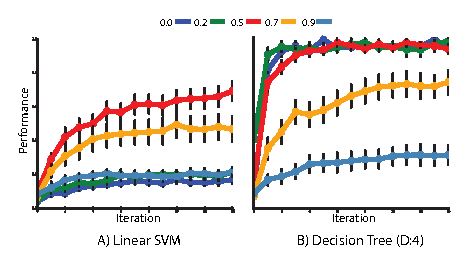
\includegraphics{f_figs/sweeping_eps.eps}
\caption{
    \footnotesize
In this experiment, we varied the choice of a fixed noise parameter, $\epsilon$. We are interested in seeing how the best $\epsilon$ varies for different learners. In A, the Linear SVM have test error, $X$ and subsequently the best $\epsilon = 0.5$. In B, the depth $4$ decision trees have test error $Y$ and the best $\epsilon$ is between $0.2$. Thus suggesting lower test error requires less injected noise. }
\vspace*{-20pt}
\label{fig:sweeep_eps}
\end{figure}




\subsubsection{Batch Learning with INIT}
In this experiment, we will try to iteratively optimize for the best value of $\epsilon$ and explore how varying the batch size $M$ effects the two on-policy and off-policy algorithms. We will optimize over batch sizes $M=10$ and $M=20$. We will consider a learner of decision tree with depth of $3$, which is different than the previously swept over learners. 


We are interested in seeing how batch size effects the algorithms. We thus remove the variable of how many samples are needed to estimate $E_{p(\tau|\theta)} J(\theta,\theta^*,\tau)$, which is an additional $5$ samples per iteration for INIT. In Sec \ref{sec:driving}, we will show for a challenging task this number of samples is negligible for performance. We set $\hat{\epsilon}_0 = 0.6$, because we expect a higher error for a shallower decision tree. 
 
 Our results, shown in Fig. \ref{fig:batch_size}, suggest that as the batch size grows DAgger is  affected in performance, however our off-policy algorithm remains unaffected. We attribute this to the fact that the current agent's distribution, $p(\tau|\theta_p)$ , becomes a worse prior for $p(\tau|\theta_P)$ as the batch size grows. However by sampling from $p(\tau|\theta^*,\epsilon)$, we are placing a conservative prior over the distribution the agent is trying to converge towards.


\begin{figure}
\centering
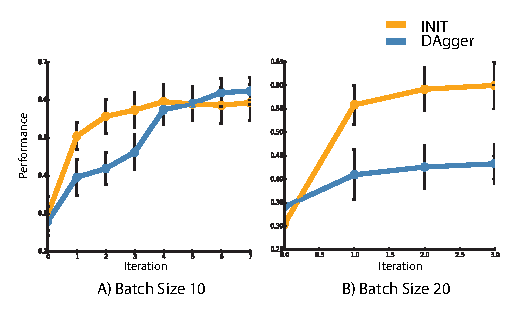
\includegraphics{f_figs/batch_size.eps}
\caption{
    \footnotesize
We demonstrate our off-policy algorithm, INIT, against a common on-policy algorithm, DAgger. In A, the amount of demonstration each learner receives is $M=10$. With small batch sizes INIT shows a slight performance win in early iterations. In B, we set the batch size to $M=20$. INIT maintains a similar performance, but DAgger suffers significantly from sampling the current agent's policy.  }
\vspace*{-20pt}
\label{fig:batch_size}
\end{figure}


\subsubsection{INIT's Sensitivity to Initialization} 
We will now examine how sensitive INIT is to the selection of $\hat{\epsilon}_0$.  We also plot the performance of the chosen $\hat{\epsilon}_0$ if it is held fixed at each iteration. Ideally, we would want INIT to provide robustness to this parameter and lead the agent to converge to a good policy. We chose a batch size of $M=10$ and used a Linear SVM as the policy class. 

The results, shown in Fig. \ref{fig:r_init}, illustrates that INIT becomes more robust to the selection of $\hat{\epsilon}_0$ as the number of iterations increases. Furthermore, it appears that INIT's adaptivity does help considering that it converges to near the second best value of the fixed noise terms for all initial noise terms. We note that that there does exists one fixed $\epsilon$, which is $0.5$ that converges to a higher value than INIT.  Thus, if an application allows for exhaustive grid-search of the parameters it may be beneficial. 


\begin{figure}
\centering
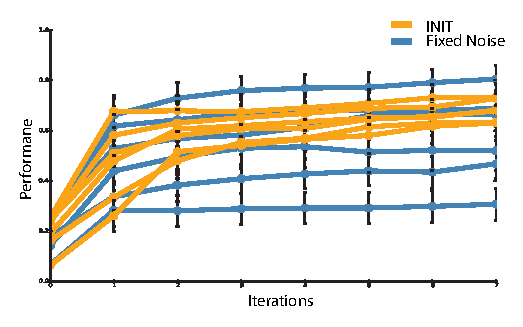
\includegraphics{f_figs/random_parameter.eps}
\caption{
We vary the initial parameter $\hat{\epsilon}_0$ that INIT requires. As the number of iterations increased the agent's trained with a different initial parameter converge in performance. We also compare INIT to selection of a fix $\epsilon$. The fixed version is not as robust to the selection of $\epsilon$, however there does exist one term $\epsilon = 0.5$ that does better than INIT. Thus suggesting adaptivity is not as good as exhaustive grid-search techniques. 
    \footnotesize}
\vspace*{-20pt}
\label{fig:r_init}
\end{figure}


\subsection{Driving Simulator}\label{sec:driving}
\mlnote{Still editing this section}
In order to test our method in situations with very large variance. We developed a driving simulator, in which the agent's car is placed on the road and must learn to drive around other vehicles. The other vehicles are randomly placed on the road at each iteration, thus the agent must learn a policy that can move around vehicles in unseen configurations. 

\mlnote{need dynamics info}

The state space of the simulator are  gray-scaled images of the workspace, which lie in the space of $S = [0,255]^{128\times128}$. The action space of the car is the selection of a steering angle for the car $A = [-30^\circ, -15^\circ, 0^\circ, 15^\circ, 30^\circ]$.

In order to ensure, consistent quality of labels in each part of the state space, the supervisor is an $A^*$  planner that has access to the internal dynamics of the game engine and a lower dimensional state space. Due to noise in the dynamics, the planner operates on the expected state. 

Our nerual net architecture consisted of a conluolutional layer and two full connected layers, seperated by ReLus. \mlnote{more detail} The architecture designed was inspired by that used in \cite{laskeyrobot}. The network was trained using TensorFlow on a Tesla K-40 GPU. 

Each roll-out of a policy take $5$s, where the majority of the computation comes from the supervisor's planner. In order to produce a large amount of data, we parrellized each roll-out on a 12 core CPU \mlnote{get infr}. 

Do to the time requirement of training a network and the ability of  to parrellize data collection, we are interested in working with a large batch size of data (i.e. $M = 150$) for $X$ iterations. We will choose $I=10$ for the policy evaluation step of INIT. 

In this experiment, we will compare DAgger, Deterministic Off-Policy, and INIT. We are also interested in comparing against an intermediate between DAgger and INIT. \mlnote{write about other methods}.

The $\beta$ parameter and $\hat{\epsilon}_)$ are tuned via grid-search where we evaluate the agent's performance after one iteration of each algorithm. 

Results suggest $X$


\begin{enumerate}
\item best Dagger on batch 
\item 50/50 mix DAgger
\item INIT
\item TRPO
\end{enumerate}
\subsubsection{Large Scale Learning}

\section{Conclusion} 

\begin{theorem}
(Ross and Bagnell 2011) Denote $ p* = \underset{p\in{1,P}}{\mbox{argmin}} E_{p(\tau|\theta_p)} J(\theta,\theta^*,\tau)$, the following inequality holds: 

$$E_{p(\tau|\theta_{p^*})} J(\theta_{p^*},\theta^*,\tau) \leq \frac{1}{P} \sum^{P-1}_{p=0} E_{p(\tau|\theta_{p^*})} J(\theta,\theta^*,\tau) + \gamma_P$$
 
\end{theorem}

\label{sec:conclusion}

The conclusion goes here.

\section*{Acknowledgments}

\section*{Appendix}

\begin{lemma}
For two deterministic agents with distributions on trajectories $p(\tau|\theta)$ and $p(\tau|\hat{\theta})$ the following inequality holds:
$$||p(\tau|\theta) - p(\tau|\hat{\theta})||_{TV}  \leq$$ $$ T\sqrt{1 - E_{p(\tau|\theta^*)} \mathbbm{1}(J)^2} $$

where $E_{p(\tau|\hat{\theta})} \mathbbm{1}(J) =  E_{p(\tau|\hat{\theta})} \mathbbm{1}(J(\theta,\hat{\theta},\tau) == 0)$ or the expected number of trajectories where the two agents apply the same controls for all states. \\
\end{lemma}

\begin{proof}
We begin our proof by restating Le Cam's Inequality, which bounds the Total Variational Distance  by the Hellinger Distance, $\mathcal{H}(p(\tau|\theta) || p(\tau|\hat{\theta}))$ on two distributions

\begin{align}
&||p(\tau|\theta) - p(\tau|\hat{\theta})||_{TV} \leq \nonumber \\
&\mathcal{H}(p(\tau|\theta) || p(\tau|\hat{\theta}))\sqrt{1-\frac{\mathcal{H}^2(p(\tau|\theta) || p(\tau|\hat{\theta}))}{4}}\nonumber
\end{align}

We will now leverage Lemma \ref{lem:hellinger_exp} to write the Hellinger distance squared as a function of an expectation over $p(\tau|\hat{\theta})$
\begin{align}
&\mathcal{H}^2(p(\tau|\theta)||p(\tau|\hat{\theta})) = 2\big(1-E_{p(\tau|\hat{\theta})} \sqrt{\frac{\prod^{T-1}_{t=0} p(a_t|\bs_t,\theta)}{\prod^{T-1}_{t=0} p(a_t|\bs_t,\hat{\theta})}}\big) \nonumber \\
&= 2(1-E_{p(\tau|\hat{\theta})} \mathbbm{1}(J(\theta,\hat{\theta},\tau) == 0))
\end{align}


The final line follows from computing the expectation over measurable trajectories under $p(\tau|\hat{\theta})$ and noting that the inner product term is $1$ when they agree and $0$ when they disagree. We then plug this term back into the original Le Cam's Inequality and simplify to obtain the bound. 
\end{proof}

\begin{theorem}
Denote $\pi_{\theta}$ a policy found using Off-Policy IL with a deterministic supervisor, the following inequality holds:
$$ |E_{p(\tau|\theta)} J(\theta,\theta^*,\tau)  - E_{p(\tau|\theta^*)} J(\theta,\theta^*,\tau) | \leq \: $$
$$ T\sqrt{1 - E_{p(\tau|\theta^*)} \mathbbm{1}(J)^2} $$
\end{theorem}

\begin{proof}
For this proof we will write  $J(\tau;\theta)$ as $J(\tau)$ and $p(\tau|\theta^*)$ as $p(\theta^*)$ for brevity. 

We first bound the difference between expectations using Lemma \ref{lem:tv_dist}. 
\begin{align}
&|E_{p(\tau|\theta)} J(\tau) - E_{p(\tau|\theta^*)} J(\tau)| =\\
&\leq T||p(\tau|\theta) - p(\tau|\theta^*)||_{TV}\\ 
 \end{align}

We then apply Lemma \ref{sec:dist_mistmatch} to obtain the proof.  
 
\end{proof}

\begin{theorem}
Denote $\pi_{\theta}$ a policy found using Off-Policy IL with an $\epsilon$-greedy strategy, the following inequality holds:
Denote $\pi_{\theta}$ a policy found using Off-Policy IL with an $\epsilon$-greedy strategy, the following inequality holds:
$$ |E_{p(\tau|\theta)} J(\theta,\theta^*,\tau)  - E_{p(\tau|\theta^*)} J(\theta,\theta^*,\tau) | \leq \: $$
$$ T\sqrt{1 - E_{p(\tau|\theta^*)}f(\epsilon,\theta^*)\mathbbm{1}(\bar{J}(\theta,\tau)))^2} $$

$$f(\epsilon,\theta^*) = ((\frac{\epsilon}{K-1})^{J(\theta,\theta^*,\tau)}(1-\epsilon)^{T-J(\theta,\theta^*,\tau)})^{-0.5}$$

where $\mathbbm{1}(\bar{J}(\theta,\tau)) =  \mathbbm{1}(\sum^T_{t=1} l(\pi_{\theta}(\bs_{t}),a_t)=0)$, or is $1$ when the agent agrees with the trajectory $\tau$. 
\end{theorem}

\begin{proof}
We first bound the difference between expectations using Lemma \ref{lem:tv_dist}. 
\begin{align}
&|E_{p(\tau|\theta)} J(\tau) - E_{p(\tau|\theta^*)} J(\tau)| =\\
&\leq T||p(\tau|\theta) - p(\tau|\theta^*)||_{TV}\\ 
 \end{align}
 
 We now apply Le Cam's Inequality to bound the total variational distance. 
 \begin{align}
&||p(\tau|\theta) - p(\tau|\hat{\theta})||_{TV} \leq \nonumber \\
&\mathcal{H}(p(\tau|\theta) || p(\tau|\theta^*))\sqrt{1-\frac{\mathcal{H}^2(p(\tau|\theta) || p(\tau|\theta^*))}{4}}\nonumber
\end{align}

We will now leverage Lemma \ref{lem:hellinger_exp} to write the Hellinger distance squared as a function of an expectation over $p(\tau|\hat{\theta})$
\begin{align}
&\mathcal{H}^2(p(\tau|\theta)||p(\tau|\theta^*)) = 2\big(1-E_{p(\tau|\theta^*)} \sqrt{\frac{\prod^{T-1}_{t=0} p(a_t|\bs_t,\theta)}{\prod^{T-1}_{t=0} p(a_t|\bs_t,\theta^*)}}\big) \nonumber 
\end{align}

We now leverage the fact that the agent is determinstic and thus 
$\prod^{T-1}_{t=0} p(a_t|\bs_t,\theta) = \mathbbm{1}(\sum^T_{t=1} l(\pi_{\theta}(\bs_{t}),a_t)=0)$ or is 1 when the agent perfectly agrees with that trajectory and 0 otherwise. 

Since we know the numerator is only non-zero when the agent agrees perfectly with the controls, we can write the denominator in terms of the surrogate loss: $\prod^{T-1}_{t=0} p(a_t|\bs_t,\theta) = (\frac{\epsilon}{K-1})^{J(\theta,\theta^*,\tau)}(1-\epsilon)^{T-J(\theta,\theta^*,\tau)}$. 

Combining these terms and simplifying yields the proof. 
\end{proof}


\begin{lemma}\label{lem:tv_dist}
Let $P$ and $Q$ be any distribution on $\mathcal{X}$. Let $f:\mathcal{X} \rightarrow [0,B]$. Then
$$|E_{P}[f(x)] - E_Q[f(x)]| \leq B ||P-Q||_{TV}$$
\end{lemma}

\begin{proof}
\begin{align}
&|\sum_x p(x)f(x) - \sum_x q(x)f(x)| \nonumber \\
&= |\sum_x (p(x)-q(x))f(x)|  \nonumber \\
&=|\sum_x (p(x)-q(x))f(x)|(f(x) - \frac{B}{2}) + \frac{B}{2}(\sum_x p(x) - q(x))| \nonumber \\
&\leq \sum_x |p(x)-q(x)||f(x) - \frac{B}{2}| \nonumber \\
&\leq \frac{B}{2} \sum_x |p(x)-q(x)|\nonumber \\
& \leq B ||P-Q||_{TV}
\end{align}

The last line applies the definition of total varaitional distance, which is $||P-Q||_{TV} = \frac{1}{2} \sum_x |p(x)-q(x)|$.

\end{proof}
%% Use plainnat to work nicely with natbib. 

\begin{lemma}\label{lem:hellinger_exp}
For two distributions on trajectories $p(\tau|\theta)$ and $p(\tau|\hat{\theta})$. Then

$$\mathcal{H}^2(p(\tau|\theta)||p(\tau|\hat{\theta})) = 2\big(1-E_{p(\tau|\hat{\theta})} \sqrt{\frac{\prod^{T-1}_{t=0} p(a_t|\bs_t,\theta)}{\prod^{T-1}_{t=0} p(a_t|\bs_t,\hat{\theta})}}\big)$$

where $\mathcal{H}^2(p(\tau|\theta)||p(\tau|\hat{\theta}))$ is the squared Hellinger distance. 

\end{lemma}

\begin{proof}
\begin{align}
&\mathcal{H}^2(p(\tau|\theta) || p(\tau|\hat{\theta})) = \nonumber\\ 
&=\sum^M_{m=0} \big(\sqrt{p(\tau_m|\theta)} - \sqrt{p(\tau_m|\hat{\theta})} \big)^2 \nonumber \\ 
&=\sum^M_{m=0} p(\tau_m|\theta) + \sum^M_{m=0} p(\tau_m|\hat{\theta}) - 2 \sum^M_{m=0} \sqrt{p(\tau_m|\theta)p(\tau_m|\hat{\theta})} \nonumber \\
& = 2\big(1 - \sum^M_{m=0} \sqrt{p(\tau_m|\theta)p(\tau_m|\hat{\theta})} \big)\\
& =  2\big(1 - \sum^M_{m=0} p(\tau_m|\hat{\theta})\sqrt{\frac{p(\tau_m|\theta)}{p(\tau_m|\hat{\theta})} }\big)\\
&= 2\big(1-E_{p(\tau|\hat{\theta})} \sqrt{ \frac{\prod^{T-1}_{t=0} p(a_t|\bs_t,\theta)}{\prod^{T-1}_{t=0} p(a_t|\bs_t,\hat{\theta})}}\big)
\end{align}
\end{proof}

\bibliography{references}
\bibliographystyle{icml2017}



\end{document}


